\section{Modelando problemas de controladores dinámicamente actualizables}

Agregamos un conjunto de palabras reservadas a FSP para poder soportar objetivos actualizables. En la figura
\ref{MTSA_example} mostramos el código FSP necesario para síntesis de controladores actualizables para el ejemplo del reactor nuclear
presentado en la sección \ref{power_plant}.

El operador \texttt{\textbf{updatingController}} es utilizado para definir el problema de controladores
actualizables. Al ejecutar la composición en paralelo de este elemento obtendremos, si existe, un controlador que satisface los
objetivos del problema de control sin violar la especificación del ambiente de actualización. Ambos definidos en el
capítulo \ref{updating_controller_chapter}. Necesitamos en esta declaración, además de los nuevos requerimientos, suministrar
el controlador actual, el modelo del ambiente actual, el modelo del ambiente nuevo y un conjunto de pares de fluents
donde cada elemento indicará correspondencia de propiedades del ambiente actual al ambiente nuevo como dijimos en la
definición \ref{update_environment_def}. Por ejemplo, en la figura \ref{MTSA_example} podemos observar que al usar la
palabra reservada \texttt{\textbf{updatingController}} configuramos \textsc{EnvironmentAndController} como el
controlador actual, \textsc{OldEnvironment} como modelo del ambiente actual, \textsc{NewEnvironment} como modelo del
ambiente nuevo, \textsc{UpdateSpec} como el conjunto de objetivos para controladores actualizables según la
definición \ref{update_goals_def} y \textsc{\{\{RequestPending,RequestPending\},
\{IsStopped,IsStopped\}\}} es el conjunto de pares de fluents donde se indica que por cada estado del ambiente actual,
existe una correspondencia con estados del ambiente nuevo si la valuación de los fluents de los primeros en cada par,
iguala a la valuación de los segundos en cada par. Además, en este ejemplo, \textsc{OldEnvironment} y
\textsc{NewEnvironment} poseen distintos nombres, pero son el mismo ambiente puesto a que este ejemplo es una
actualización que no requiere hacer un cambio en el ambiente.

Los objetivos nuevos están definidos mediante el operador \texttt{\textbf{controllerSpec}}. La palabra reservada
\texttt{\textbf{safety}} permite definir requerimientos de seguridad (\emph{safety}). Aquí incluiremos fórmulas
FLTL definidas en la sección \ref{LTL} y, en particular para controladores actualizables dinámicamente, escribiremos las
fórmulas FLTL 1, 2 y 3 de acuerdo a la definición \ref{update_goals_def}. Como se puede ver en la figura \ref{MTSA_example},
\textsc{UPD\_OLD} representa la fórmula 1, \textsc{UPD\_NEW} corresponde a la fórmula 2 y la fórmula 3 no está
especificada debido a que en este ejemplo configuramos a la fórmula 3 como $true$. \textsc{S\_OLD} y \textsc{S\_NEW} son
aserciones FLTL que representan a los objetivos viejos ($G$) y a los objetivos nuevos ($G'$) respectivamente.

\begin{figure}
    \centering
    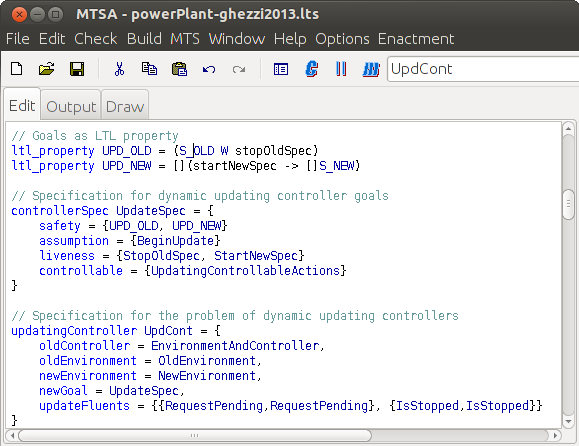
\includegraphics[scale=0.35]{img/MTSA_example.png}
    \caption{MTSA -- Definición de problema de controladores dinámicamente actualizables}
    \label{MTSA_example}
\end{figure}

La sección de \emph{liveness} esta definida usando los operadores \texttt{\textbf{assumption}} y
\texttt{\textbf{liveness}} que especifican las asunciones del ambiente y objetivos de \emph{liveness} respectivamente.
Ambas deberán definirse mediante FLTLs. En la figura \ref{MTSA_example}, \textsc{BeginUpdate}, \textsc{StopOldSpec} y
\textsc{StartNewSpec} son los fluents que se inicializan apagados y se prenden cuando la acción del nombre del fluent
sucede y nunca más se apagarán. Luego, el controlador sintetizado nos garantizará que si la actualización es requerida
(i.e sucede la acción $beginUpdate$), las acciones $stopOldSpec$ y $startNewSpec$ sucederán. Por lo tanto,
con estos dos operadores definimos las fórmula 4 y 5 de la definición \ref{update_goals_def}.

Por último, la sección de \texttt{\textbf{controllableActions}} detalla el conjunto de acciones consideradas
controlables a la hora de resolver el problema de control. En nuestro ejemplo, utilizamos a
\textsc{UpdatingControllableActions} que posee las acciones $stopPump$, $startPump$, $procedure$ y $ok$ que son las
acciones controlables del controlador original; y $startNewSpec$ y $stopOldSpec$ que son los eventos especiales
agregados para resolver el problema de controladores actualizables dinámicamente.




